\pagebreak
\section{Auswertung}

\subsection{Verifizierung der Funktionsweise des Lock-In-Verstärkers}
\subsubsection{Ohne Rauschsignal}
In den folgenden Abbildungen \eqref{fig:klar1}, \eqref{fig:klar2}, \eqref{fig:klar3}, \eqref{fig:klar4} und \eqref{fig:klar5} sind die Spannungen bei Phasenverschiebungen von 0°, 15°, 30°, 45° und 60° zu sehen. 

\begin{figure}[h!tbp]
	\centering
	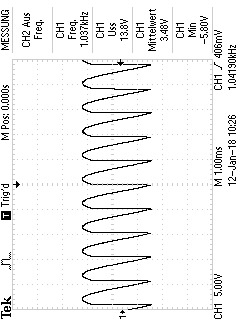
\includegraphics[angle=-90, width=0.5\linewidth]{klar1.jpeg}
	\caption{Spannungssignal bei einer Phase von 0°. }
	\label{fig:klar1}
\end{figure}

\begin{figure}[h!tbp]
	\centering
	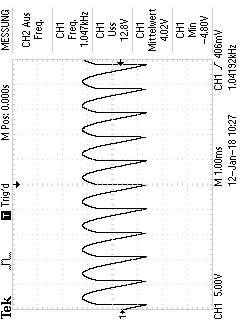
\includegraphics[angle=-90, width=0.5\linewidth]{klar2.jpeg}
	\caption{Spannungssignal bei einer Phase von 15°. }
	\label{fig:klar2}
\end{figure}

\begin{figure}[h!tbp]
	\centering
	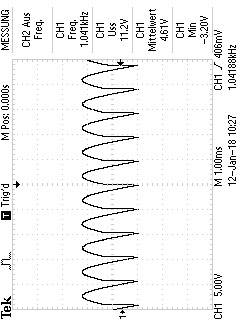
\includegraphics[angle=-90, width=0.5\linewidth]{klar3.jpeg}
	\caption{Spannungssignal bei einer Phase von 30°. }
	\label{fig:klar3}
\end{figure}

\begin{figure}[h!tbp]
	\centering
	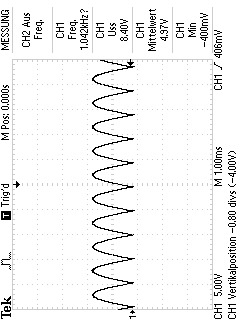
\includegraphics[angle=-90, width=0.5\linewidth]{klar4.jpeg}
	\caption{Spannunggssignal bei einer Phase von 45°. }
	\label{fig:klar4}
\end{figure}

\begin{figure}[h!tbp]
	\centering
	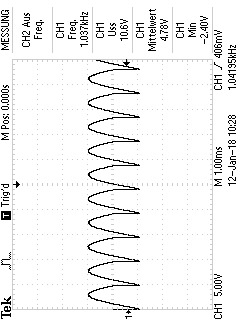
\includegraphics[angle=-90, width=0.5\linewidth]{klar5.jpeg}
	\caption{Spannungssignal bei einer Phase von 60°. }
	\label{fig:klar5}
\end{figure}

\newpage
Zudem können aus Tabelle \eqref{tab:phaseundspannung} die gemessenen Ausgangsspannungen zu zehn verschiedenen Phasen entnommen werden und sind weiterhin in Abbildung \eqref{fig:klarewerte} gegeneinander aufgetragen.
\begin{table}[h!tbp]
   \centering
   \caption{Messdaten von Phasenverschiebung und Spannung, ohne Rauschsignal.}
   \label{tab:phaseundspannung}
   \begin{tabular}{
S[table-format=3.0, table-auto-round] 
S[table-format=2.1, table-auto-round]
}
\toprule
{$\phi/\,\symup{Grad}$} & {$U/10^{-3}\,\symup{V}$} \\
\midrule
0  & 1.25 \\
30 & -30.4  \\
60  & -66.4 \\
90  & -72.6 \\
120  & -64.5 \\
150  & -29.1 \\
180 & 1.62 \\
210 & 32.3 \\
240 & 67.3 \\
270 & 73.1 \\

\bottomrule
\end{tabular}
\end{table}

\begin{figure}[h!tbp]
	\centering
	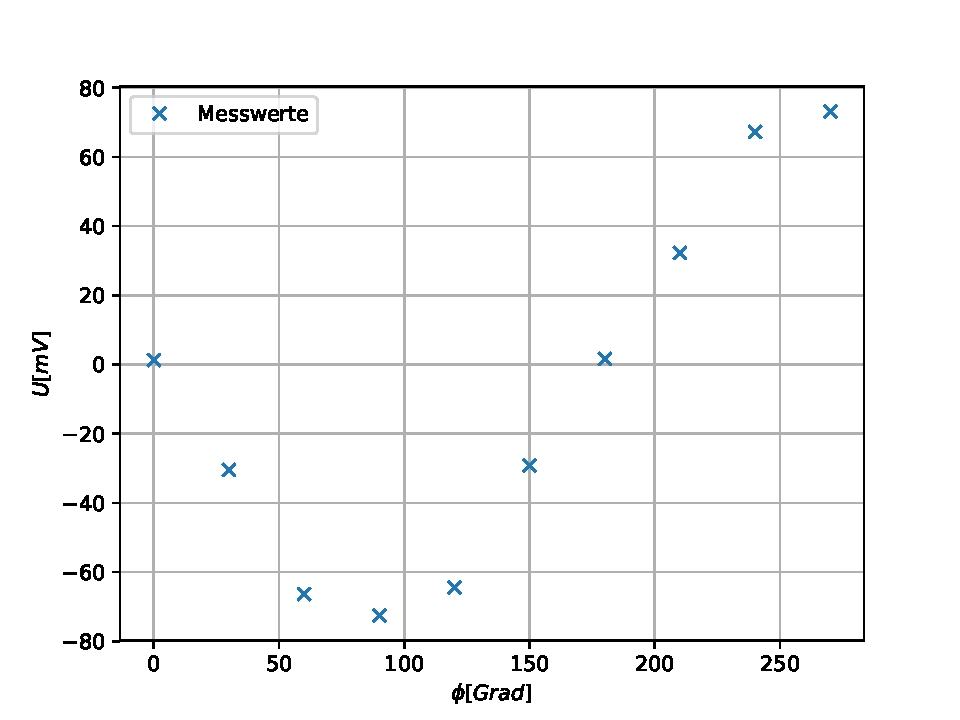
\includegraphics[width=0.9\linewidth]{klarewerte.pdf}
	\caption{Spannung in Abhängigkeit der Phasenverschiebung, ohne Rauschsignal. }
	\label{fig:klarewerte}
\end{figure}





\pagebreak
\newpage
\subsubsection{Mit Rauschsignal}
Die Messungen werden mit einem durch ein Noise Generator erzeugtes Rauschsignal wiederholt. Es ergeben sich die in \eqref{fig:rausch1}, \eqref{fig:rausch2}, \eqref{fig:rausch3}, \eqref{fig:rausch4}, 
\eqref{fig:rausch5} zu sehenden Bilder.

\begin{figure}[h!tbp]
	\centering
	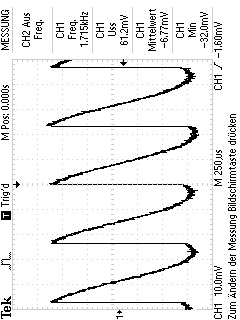
\includegraphics[angle=-90, width=0.5\linewidth]{rausch1.jpeg}
	\caption{Spannungssignal bei einer Phase von 0°. }
	\label{fig:rausch1}
\end{figure}

\begin{figure}[h!tbp]
	\centering
	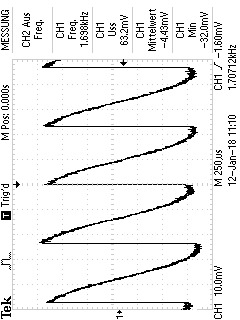
\includegraphics[angle=-90, width=0.5\linewidth]{rausch2.jpeg}
	\caption{Spannungssignal bei einer Phase von 15°. }
	\label{fig:rausch2}
\end{figure}

\begin{figure}[h!tbp]
	\centering
	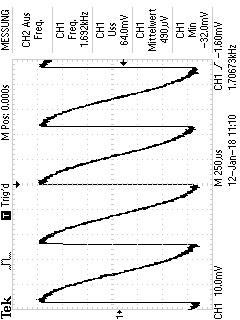
\includegraphics[angle=-90, width=0.5\linewidth]{rausch3.jpeg}
	\caption{Spannungssignal bei einer Phase von 30°. }
	\label{fig:rausch3}
\end{figure}

\begin{figure}[h!tbp]
	\centering
	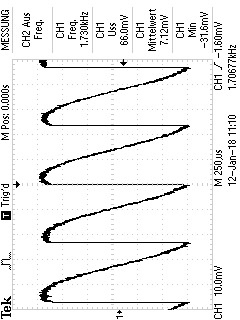
\includegraphics[angle=-90, width=0.5\linewidth]{rausch4.jpeg}
	\caption{Spannungssignal bei einer Phase von 45°. }
	\label{fig:rausch4}
\end{figure}

\begin{figure}[h!tbp]
	\centering
	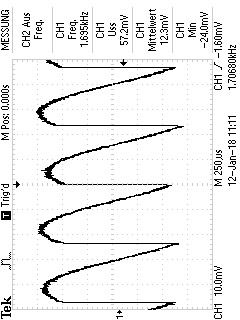
\includegraphics[angle=-90, width=0.5\linewidth]{rausch5.jpeg}
	\caption{Spannungssignal bei einer Phase von 60°. }
	\label{fig:rausch5}
\end{figure}

\pagebreak

In dieser Messreihe wurden die folgenden Werte für Phasenverschiebung und Spannung genommen:
\begin{table}[h!tbp]
   \centering
   \caption{Messdaten von Phasenverschiebung und Spannung, mit Rauschsignal.}
   \label{tab:phaseundspannungrauschen}
   \begin{tabular}{
S[table-format=3.0, table-auto-round] 
S[table-format=2.1, table-auto-round]
}
\toprule
{$\phi/\,\symup{Grad}$} & {$U/10^{-3}\,\symup{V}$} \\
\midrule
0  & -13.3 \\
30 & 3.88  \\
60  & 26.9 \\
90  & 35.4 \\
120  & 38.4 \\
150  & 28.9 \\
180 & 14.6 \\
210 & -2.07 \\
240 & \\
270 &  \\

\bottomrule
\end{tabular}
\end{table}

\begin{figure}[h!tbp]
	\centering
	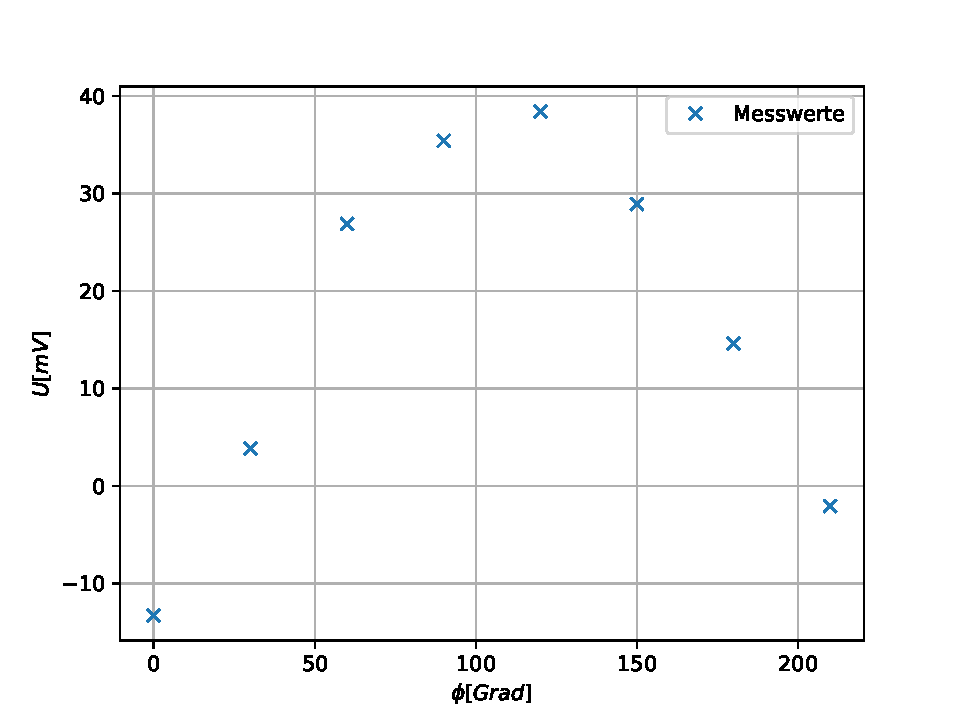
\includegraphics[width=0.9\linewidth]{rauschwerte.pdf}
	\caption{Spannung in Abhängigkeit der Phasenverschiebung, mit Rauschsignal. }
	\label{fig:rauschwerte}
\end{figure}






\subsection{Überprüfen der Rauschunterdrückung mit einer Photodetektorschaltung}
Die Werte für die eingestellten Abstände $r$ sowie die abgelesenen Spannungen $U$ sind in der nachfolgenden Tabelle zu finden.
 \begin{table}[h!tbp]
   \centering
   \caption{Messdaten von Abstand und Spannung.}
   \label{tab:messdatenphotodetektor}
   \begin{tabular}{
S[table-format=2.1, table-auto-round] 
S[table-format=3.2, table-auto-round]
}
\toprule
{$r/\,\symup{cm}$} & {$U/10^{-3}\,\symup{V}$} \\
\midrule
2.6  & 243.00 \\
4.6 & 100.00  \\
6.6  & 51.5 \\
8.6  & 23.6 \\
9.6  & 19.5 \\
10.6  & 13.4 \\
12.6 & 9.06 \\
14.6 & 7.9 \\
16.6 & 7.04\\
18.6 & 5.33\\
20.6 & 4.4\\
22.6 & 4.05\\
24.6 & 3.83\\
26.6 & 3.6\\ 
28.6 & 3.35\\
30.6 & 3.22\\
35.6 & 2.7\\
40.6 & 2.36\\
45.6 & 2.07\\
55.6 & 1.8\\
65.6 & 1.65\\

\bottomrule
\end{tabular}
\end{table}


Die Werte werden, wie in Abbildung \eqref{fig:diode} zu sehen, gegeneinander aufgetragen.
\begin{figure}[h!tbp]
	\centering
	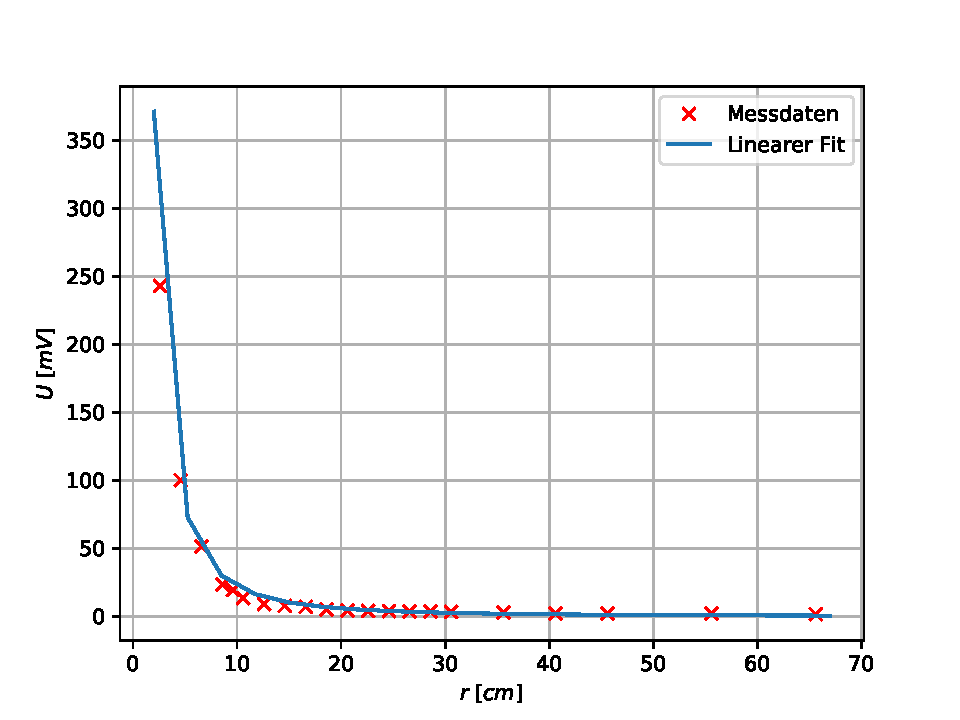
\includegraphics[width=0.9\linewidth]{diode.pdf}
	\caption{Spannung in Abhängigkeit des Abstands. }
	\label{fig:diode}
\end{figure}

\pagebreak
Vom Python-Modul Matplotlib wird eine Ausgleichskurve der Form $y = \frac{a}{(r+b)^2}$ angelegt. Ebenso berechnet es für $a$ und $b$:
\begin{equation*}
\begin{aligned}
a &= 2477{,}3 \pm 151{,}5 \\
b &= 0{,}583 \pm 0{,}104 \\
\end{aligned}
\end{equation*}

Zum Ende hin ist die Steigung der Ausgleichkurve näherungsweise konstant, sodass $r_{\text{max}}$, also der Abstand ab dem das Licht der Diode nicht mehr zu der gemessenen Lichtintensität beiträgt, hier auf
\begin{equation*}
r_{\text{max}} = 65{,}6\,\symup{cm}
\end{equation*}
gesetzt werden kann. 




